\documentclass[preprint,12pt]{elsarticle}
\usepackage[utf8]{inputenc}
\usepackage[T1]{fontenc}
\usepackage{lmodern}
\usepackage{amsmath,amssymb,amsfonts}
\usepackage{graphicx}
\usepackage{booktabs}
\usepackage{longtable}
\usepackage{array}
\usepackage{tabularx}
\usepackage{geometry}
\usepackage{url}
\usepackage{hyperref}
\usepackage{float}
\usepackage{placeins}
\geometry{margin=1in}
\graphicspath{{paper/}{paper/figures/}{figures/}}
\hypersetup{colorlinks=true,linkcolor=black,citecolor=blue,urlcolor=blue,hypertexnames=false}
\urlstyle{same}
\setlength{\emergencystretch}{2em}
\makeatletter
\pdfstringdefDisableCommands{\def\corref#1{}\def\@corref#1{}\def\cnotenum#1{}}
\makeatother
\journal{Journal of Computational Science}
\makeatletter
\long\def\pprintMaketitle{\clearpage
  \iflongmktitle\if@twocolumn\let\columnwidth=\textwidth\fi\fi
  \resetTitleCounters
  \def\baselinestretch{1}%
  \printFirstPageNotes
  \begin{\elsarticletitlealign}%
 \thispagestyle{pprintTitle}%
   \def\baselinestretch{1}%
    \Large\@title\par\vskip18pt%
    \ifx\@elsarticlenewpageafter\newpage@after@title%
      \newpage
    \fi%
    \ifdoubleblind
      \vspace*{2pc}
    \else
      \normalsize\elsauthors\par\vskip10pt
      \footnotesize\itshape\elsaddress\par\vskip36pt
    \fi
    \ifx\@elsarticlenewpageafter\newpage@after@author%
      \newpage
    \fi%
    \ifvoid\absbox\else\unvbox\absbox\par\vskip10pt\fi
    \ifvoid\keybox\else\unvbox\keybox\par\vskip10pt\fi
    \ifx\@elsarticlenewpageafter\newpage@after@abstract%
      \newpage
    \fi%
    \end{\elsarticletitlealign}%
    \gdef\thefootnote{\arabic{footnote}}%
  }
\long\def\MaketitleBox{%
  \resetTitleCounters
  \def\baselinestretch{1}%
  \begin{\elsarticletitlealign}%
   \def\baselinestretch{1}%
    \Large\@title\par\vskip18pt
  \ifdoubleblind
    \vspace*{2pc}
  \else
    \normalsize\elsauthors\par\vskip10pt
    \footnotesize\itshape\elsaddress\par\vskip36pt
  \fi
    \ifvoid\absbox\else\unvbox\absbox\par\vskip10pt\fi
    \ifvoid\keybox\else\unvbox\keybox\par\vskip10pt\fi
    \end{\elsarticletitlealign}%
}
\makeatother

\begin{document}
\begin{frontmatter}
\title{A Model-Conditioned Attribution Protocol for Graph Priors in Node-Wise Scientific Latent Dynamics}
\begin{abstract}

Graph-prior gains in scientific latent dynamics are often reported as
prediction improvements, but such gains do not by themselves show that
the model used the candidate graph topology. We propose a
model-conditioned attribution protocol that decomposes graph-prior
efficacy into four operational protocol outcomes: (i) controlled
audit-positive / topology-aligned support, requiring agreement between
rollout point-estimate ordering and audit-mode latent-metric
separation against topology-breaking controls; (ii) topology-specific
rollout support, a rollout-only outcome reserved for standard cells
that separate from matched controls; (iii) generic regularization,
where graph priors show graph-vs-none utility or practical gain but
the gains do not survive topology-breaking controls; and (iv) no
effect. Across
13 measurement cells of heterogeneous evidential strength, including
12 replicated cells and one graph-heat legacy single-seed cautionary
cell, the protocol identifies 1 controlled audit-positive /
topology-aligned support cell, 0 topology-specific rollout-support
cells, 8 generic-regularization cells, and 4 no-effect cells. The
generic-regularization block spans N-body synthetic data and 3-seed
historical Cycle-2 rMD17 corroborating evidence without a calibrated
temporal-smoothing arm. Across the
eight generic-regularization cells, graph-arm-SEM-normalized
improvements against the no-prior baseline range from 2.4 to 8.4,
while the same diagnostic against the SMPG control ranges from \(-2.9\)
to \(0.9\) with confidence-interval overlap in every cell. Thus,
graph-vs-none improvements in our evidence would have been
over-attributed without SMPG controls. The protocol is offered as a
practical attribution-control workflow for prior selection and
interpretation under a fixed model condition.

\end{abstract}
\end{frontmatter}

\section{Introduction}

Scientific dynamics models increasingly combine learned latent-state evolution with auxiliary priors motivated by domain structure. In molecular dynamics, coupled oscillator systems, particle simulations, traffic networks, and graph-discretized physical fields, observations can often be written as trajectories $X_t$ over $N$ interacting nodes. Before fitting a full model, a practitioner may already have a plausible candidate graph, a temporal smoothness assumption, or another regularizer that appears scientifically reasonable. Such priors are attractive because they may stabilize long-horizon rollout prediction, improve sample efficiency, and encode structure that is difficult to infer from limited data alone. Their practical value, however, is not intrinsic to the prior alone. It depends on how the prior interacts with the encoder, transition model, latent dimension, prior placement, optimization setting, training budget, and rollout horizon.

In the settings tested here, this dependence makes graph-prior effects difficult to interpret. A Laplacian penalty on learned node-wise latents may improve rollout because the candidate graph captures meaningful physical or scientific structure. The same gain may also arise because the penalty imposes generic graph-frequency smoothing, because a spectrum-matched permuted graph control would have produced a similar effect, because calibrated temporal smoothing would have been sufficient, or because the apparent advantage is confined to a short budget before an unconstrained model catches up. A graph-aware encoder or transition model can further blur the interpretation by already encoding part of the relational bias. Consequently, in our evidence and protocol, a graph prior outperforming the no-prior baseline establishes practical utility but does not by itself establish topology-specific attribution.

From a computational-science perspective, this ambiguity creates an attribution problem. In our workflow, sweeps over priors, graph constructions, regularization strengths, seeds, and budgets can still leave interpretation unresolved if the comparison set is incomplete. What is often needed first is a matched-control attribution screen: should the candidate graph be interpreted as useful regularization, should a graph-free alternative be preferred, or should stronger controls be introduced before any topology-specific claim is made? We therefore frame prior choice as a preflight problem. The preflight workflow determines whether a prior is useful, what explains the gain, and what evidence would still be required before making topology-specific claims.

This article develops that idea as a model-conditioned attribution workflow for graph priors in node-wise scientific latent dynamics. The protocol compares no-prior training, a candidate graph prior, a spectrum-matched permuted graph control, optional random-graph controls, and calibrated temporal smoothing. Audit mode, used when checkpointed latent traces are available, additionally examines whether predictive gains coincide with latent behavior aligned with the candidate graph. The contribution is methodological rather than architectural: the paper introduces attribution control for prior selection and interpretation under a fixed model condition, and it uses a conservative four-outcome vocabulary to convert ambiguous prior effects into bounded claims. The boundary is intentionally local: the protocol evaluates graph-prior interpretation under the tested model condition rather than proposing a new graph architecture or benchmark leaderboard.

\section{Related Work}

This manuscript sits at the intersection of several active lines of research while remaining narrower in scope than any one of them. A first strand comes from graph signal processing and geometric deep learning, where graph Fourier structure, Laplacian smoothness, message passing, and graph-based regularizers encode relational inductive bias on non-Euclidean domains \citep{chung1997spectral,shuman2013emerging,ortega2018graph,bronstein2021geometric,kipf2017semi,gilmer2017neural,battaglia2018relational}. Prior literature establishes graph structure as useful for prediction and representation learning; our narrower question is attribution under a fixed tested protocol. This paper instead asks: under a fixed latent dynamics model, when does a candidate graph prior merit further computation, and what controls are required before topology-specific attribution is justified?

A second strand concerns scientific and physical latent dynamics models, including world-model formulations and graph-network simulators that learn compact state representations and transition operators for dynamical systems \citep{hansen2024tdmpc2,hafner2023dreamerv3,hansen2024puppeteer,sanchez2020learning}. In these settings, priors are often introduced to stabilize rollout, improve sample efficiency, or encode known structure suggested by measurement geometry or domain knowledge. The contribution here is complementary: it proposes a standardized model-conditioned attribution workflow for deciding how a candidate prior should be interpreted under a specified model condition.

A third strand includes causal, structural, and interaction-discovery work \citep{scholkopf2021toward,kipf2018nri}. That literature seeks latent variables or relational structure aligned with underlying mechanisms, and it often asks whether learned representations capture more than predictive convenience. The present manuscript adopts some of the same caution about interpretation, but its goal is narrower. The workflow compares predictive priors under matched controls and asks whether observed gains support topology-specific attribution; it does not attempt to identify a true interaction graph from data alone.

A fourth strand concerns spatiotemporal graph forecasting, molecular graph priors, and model-selection diagnostics in machine learning and computational science \citep{li2018dcrnn,yu2018stgcn,wu2019graphwavenet,schutt2018schnet,satorras2021egnn}. These approaches emphasize controlled baselines, matched comparisons, calibration, ablation, and concise reporting to guide computational decisions. The present protocol belongs most directly in this diagnostic tradition. Its emphasis is on matched prior comparisons, topology-breaking control checks, graph-free temporal controls where available, and optional audits that produce bounded attribution statements.

Random-graph or shuffled-adjacency ablations are common in graph-prior and graph-learning work, but they do not necessarily preserve the full Laplacian spectrum. The SMPG control used here is designed to separate graph-frequency smoothing from node-label topology. Likewise, graph smoothness and Dirichlet-energy diagnostics can quantify graph-signal alignment, but they do not by themselves establish predictive utility under a fixed model condition. This manuscript's narrower contribution is the combination of spectrum-preserving topology-breaking controls, graph-free temporal controls where available, optional latent audits, and conservative attribution vocabulary into one model-conditioned attribution workflow.

Taken together, these literatures motivate the need for the present study while also clarifying its boundary. This paper should be read as a prior-selection and attribution workflow for node-wise scientific latent dynamics: it draws on graph-based inductive bias, latent dynamics modeling, and diagnostic practice to prevent over-attribution of graph-vs-none gains.

\section{Problem formulation}

We consider node-wise physical or scientific trajectory data $X_{1:T}$, where each frame $X_t \in \mathbb{R}^{N\times d}$ contains $d$ observed features for each of $N$ nodes. A dataset adapter provides these trajectories, a candidate graph or graph Laplacian $L \in \mathbb{R}^{N\times N}$, and metadata describing the graph source, the underlying simulator or dataset, and whether the graph is known, approximate, constructed, or data-derived. The predictive model maps observations into learned latent node states $H_t \in \mathbb{R}^{N\times m}$ and trains a transition model to forecast future dynamics.

The relevant object for interpretation is the model condition. In this manuscript, the model condition comprises the encoder, transition model, latent dimension, prior placement, optimizer settings, prior strength, training budget, and rollout evaluation horizon. A preflight result is therefore not a dataset-level truth statement. It is a recommendation tied to the tested model condition and must be reconsidered if the architecture, prior location, regularization strength, budget, or evaluation horizon changes.

The central question is the following:

\begin{quote}
Under this model condition and training budget, does a candidate prior improve rollout prediction, and is the improvement better attributed to candidate topology, generic graph-frequency regularization, calibrated temporal smoothing, or an effect specific to the tested model condition?
\end{quote}

This formulation is intentionally narrower than causal discovery, universal physics modeling, or benchmark optimization. The objective is attribution control: avoid false topology-specific attribution, decide whether the tested evidence supports controlled audit-positive / topology-aligned support, topology-specific rollout support, generic regularization, or no effect, and state the resulting claim boundary under the fixed model condition. Throughout the reported experiments, rollout quality is evaluated at fixed horizons, with H32 serving as the principal manuscript readout.

Two non-goals follow directly from this framing. First, the protocol does not claim that a useful candidate graph is physically true. Second, it does not claim universal coverage across scientific systems. The experiments are therefore presented as representative node-wise physical/scientific dynamics regimes rather than as a universal physics prediction study.

\section{Mathematical and computational framing}

The protocol separates prior utility from topology-specific attribution by evaluating several prior families under the same model condition, with the graph-spectral viewpoint following standard references in spectral graph theory \citep{chung1997spectral}. The baseline condition is \texttt{none}, in which the latent dynamics model is trained without an auxiliary prior. The principal candidate graph prior is graph Laplacian smoothness on learned node-wise latent states. For a latent matrix $H$, the graph penalty is

\begin{equation}
R_G(H;L)=\mathrm{Tr}(H^\top L H)
\end{equation}

If $L = U \Lambda U^\top$ is the eigendecomposition of the Laplacian and $H = U A$, then

\begin{equation}
\mathrm{Tr}(H^\top L H)=\mathrm{Tr}(A^\top \Lambda A)=\sum_k \lambda_k \lVert a_k \rVert_2^2
\end{equation}

This identity clarifies why graph-prior gains require caution. The candidate graph prior penalizes high graph frequencies more strongly, so improved rollout may reflect useful scientific structure, but it may also reflect generic regularization in the graph spectral domain.

To probe that distinction, the key attribution baseline is the spectrum-matched permuted graph control. With permutation matrix $P$, the control Laplacian is

\begin{equation}
L_{\mathrm{perm}}=P^\top L P
\end{equation}

This transformation preserves the eigenvalues of $L$, and hence the scale of graph-frequency smoothing, while disrupting node-label semantics. Within this protocol, if the candidate graph prior improves over the no-prior baseline but not over the spectrum-matched permuted graph control, the evidence supports predictive smoothing rather than topology-specific attribution. Random-graph controls can be informative secondary checks, but they are weaker because they do not preserve the full Laplacian spectrum.

In the SMPG arm, the data tensor node order is held fixed and only the prior Laplacian is relabeled by \(P\). Thus the Laplacian spectrum and smoothing scale are preserved while the graph--node correspondence is intentionally broken. For the reported rollout comparisons, one trained SMPG arm is used per training seed unless otherwise stated. Some run artifacts store additional permuted-graph diagnostics; these are metadata for preflight analysis and are not counted as separate trained rollout arms in Tables~\ref{tab:headline}--\ref{tab:sem-summary}. Multiple independently trained SMPG draws are a natural extension and are listed as a limitation below, because a single trained SMPG draw may not exhaust topology-breaking nulls, especially for symmetry-rich graphs.

The protocol also includes a graph-free baseline,

\begin{equation}
R_T(H_{1:T})=\sum_t \lVert H_{t+1}-H_t \rVert_F^2
\end{equation}

which we refer to as calibrated temporal smoothing when its effective regularization scale has been matched to the candidate graph prior. Calibration is necessary because raw temporal losses can be much smaller than graph-Laplacian losses. If $\alpha_G$ denotes the graph-prior weight and $R_G^0$ and $R_T^0$ denote initial auxiliary-loss values measured under the same calibration pass, the temporal weight is chosen as

\begin{equation}
\alpha_T = \frac{\alpha_G R_G^0}{R_T^0+\varepsilon}
\end{equation}

so that

\begin{equation}
\alpha_T R_T^0 \approx \alpha_G R_G^0
\end{equation}

This calibration does not assert that graph and temporal priors are equivalent. It ensures that the comparison asks a fairer question: at matched initial regularization strength, does the candidate graph add value beyond graph-free temporal smoothing? The same framing also clarifies why, in our evidence, graph versus none alone is insufficient for topology-specific attribution. That stronger interpretation requires explicit comparison with the spectrum-matched permuted graph control and, where available, calibrated temporal smoothing.

\section{Model-conditioned preflight protocol}
\label{sec:protocol}

The model-conditioned preflight protocol is designed as a staged attribution workflow rather than a substitute for model validation. It begins with diagnostics that summarize the candidate graph and the observed dynamics, proceeds to controlled matched-prior comparisons, and uses latent audits when the available artifacts support mechanism-level interpretation.

Operationally, the workflow has four stages. First, trajectories, candidate graph metadata, and the corresponding Laplacian are loaded from a dataset adapter. Second, the prior family set is defined: \texttt{none}, the candidate graph prior, the spectrum-matched permuted graph control, optional random-graph controls, and calibrated temporal smoothing when a graph-versus-temporal comparison is needed. Third, models are trained under the fixed model condition and rollout is evaluated at fixed horizons. Fourth, if checkpointed latent traces are available, audit mode examines whether rollout gains coincide with smoother or more low-frequency latent temporal deltas in the candidate graph basis.

Tables~\ref{tab:attribution-classes} and~\ref{tab:prior-families} summarize the protocol outputs and the matched prior/control arms. The operational decision rule is defined in Section~\ref{sec:decision-rule}.

Audit mode is used when checkpointed latent traces are available; it asks whether predictive gains coincide with latent behavior aligned with the candidate graph and provides the strongest available evidence for topology-aligned support. The assignment logic is stated explicitly in Section~\ref{sec:decision-rule}: standard rollout cells are classified by graph-vs-none utility and separation from matched controls, while the HO audit is treated as a controlled audit-positive exception based on rollout point-estimate ordering plus separated latent audit metrics.

The resulting labels are listed in Table~\ref{tab:attribution-classes}, and the prior families on which they depend are summarized in Table~\ref{tab:prior-families}. Taken together, these tables define the vocabulary of the protocol and the corresponding actionable prior recommendation associated with each outcome.

\begingroup
\footnotesize
\setlength{\tabcolsep}{3pt}
\renewcommand{\arraystretch}{1.08}
\begin{longtable}{>{\raggedright\arraybackslash}p{0.20\textwidth}>{\raggedright\arraybackslash}p{0.30\textwidth}>{\raggedright\arraybackslash}p{0.23\textwidth}>{\raggedright\arraybackslash}p{0.19\textwidth}}
\caption{Operational attribution outcomes and claim boundaries}\label{tab:attribution-classes}\label{tab:protocol-labels}\\
\toprule
\textbf{operational attribution outcome} & \textbf{evidence pattern} & \textbf{recommended interpretation} & \textbf{claim boundary} \\
\midrule
\endfirsthead
\toprule
\textbf{operational attribution outcome} & \textbf{evidence pattern} & \textbf{recommended interpretation} & \textbf{claim boundary} \\
\midrule
\endhead
\midrule
\multicolumn{4}{r}{\emph{Continued on next page}} \\
\midrule
\endfoot
\bottomrule
\endlastfoot
controlled audit-positive / topology-aligned support & Graph has the best rollout point estimate among graph and topology-breaking controls, and audit-mode latent metrics separate in the topology-aligned direction. & Strongest preflight support under the tested model condition. & Controlled support, not topology discovery; does not prove the candidate graph is true. \\
topology-specific rollout support & In a standard rollout cell, graph strictly improves over no-prior and separates from SMPG, random-graph, or temporal controls where available under the CI rule, but audit traces are unavailable or audit has not yet been performed. & Rollout-level topology-specific evidence; carry to audit if available. & Not mechanism proof; current count is zero cells. \\
generic regularization & Graph shows graph-vs-none utility or practical gain, but does not separate from SMPG, random-graph, or temporal controls where available. & The graph prior is predictively useful, but topology is not identified. & Do not claim the candidate topology caused the gain. \\
no effect & Graph does not improve over no-prior or is worse on average without sufficient evidence for graph utility. & Do not carry the candidate graph forward under this model condition. & Does not prove all graph priors are useless. \\
\end{longtable}
\endgroup

\begingroup
\footnotesize
\setlength{\tabcolsep}{4pt}
\begin{longtable}{>{\raggedright\arraybackslash}p{0.15\textwidth}>{\raggedright\arraybackslash}p{0.29\textwidth}>{\raggedright\arraybackslash}p{0.27\textwidth}>{\raggedright\arraybackslash}p{0.21\textwidth}}
\caption{Prior families and attribution roles}\label{tab:prior-families}\\
\toprule
\textbf{prior family} & \textbf{definition} & \textbf{attribution role} & \textbf{manuscript use} \\
\midrule
\endfirsthead
\toprule
\textbf{prior family} & \textbf{definition} & \textbf{attribution role} & \textbf{manuscript use} \\
\midrule
\endhead
\midrule
\multicolumn{4}{r}{\emph{Continued on next page}} \\
\midrule
\endfoot
\bottomrule
\endlastfoot
\path{none} & No auxiliary prior. & Establishes whether any prior improves rollout. & Baseline for all preflight recommendations. \\
\path{graph_laplacian} & Candidate-graph Laplacian smoothness on learned node-wise latents, $\mathrm{Tr}\left(H^\top L H\right)$. & Tests whether candidate graph-frequency smoothing helps the tested model. & Main prior under evaluation, not introduced as a new prior. \\
\path{permuted_graph} & Spectrum-matched permuted Laplacian, $L_{\mathrm{perm}} = P^\top L P$. & Preserves Laplacian spectrum while removing node-label semantics. & Primary control for topology attribution in this protocol. \\
\path{random_graph} & Optional graph with matched coarse size or edge statistics. & Tests whether an unrelated graph can produce similar smoothing. & Secondary control; weaker than the spectrum-matched permuted graph control. \\
\path{temporal_smooth} & Graph-free smoothness on learned latent temporal deltas, e.g. $\sum_t \lVert H_{t+1}-H_t \rVert_F^2$. & Tests whether temporal regularization explains candidate graph gains. & Must be calibrated when compared with graph priors. \\
\end{longtable}
\endgroup

\subsection{Operational attribution rule and confidence intervals}
\label{sec:decision-rule}

For standard rollout cells, H32 rollout error is the primary readout. We summarize graph-vs-none utility using the graph mean, SEM-normalized improvement, and confidence-interval relation to the no-prior baseline. A strict graph-vs-none positive is defined by a lower graph mean together with non-overlapping 95\% confidence intervals against the no-prior baseline. In lower-seed or historical corroborating cells, such as the rMD17 Cycle-2 summaries that provide 3-seed historical Cycle-2 corroborating evidence without a calibrated temporal-smoothing arm, we also report practical graph-vs-none gains through positive SEM-normalized improvements and lower graph means, while explicitly marking when confidence intervals overlap. A cell is assigned to topology-specific rollout support only when a standard rollout graph-vs-none positive also separates from SMPG, random-graph, or calibrated temporal-smoothing controls where those controls are available; no reported standard rollout cell meets this outcome. A cell is assigned to generic regularization when the graph shows graph-vs-none utility or practical gain but does not separate from SMPG, random-graph, or calibrated temporal-smoothing controls where those controls are available. A cell is assigned to no effect when the graph does not improve over no-prior under this evidence standard, or when the graph is worse on average and the evidence does not support carrying it forward.

Unless explicitly stated otherwise, prose values written as ``mean \(\pm\) SD'' denote sample mean \(\pm\) sample standard deviation across seeds. 95\% confidence intervals are reported in brackets as \([{\rm lower}, {\rm upper}]\), or shown as error bars in figures when stated. For \(n\) seeds, 95\% confidence intervals are computed using the \(t\) distribution with \(df=n-1\). For \(n=1\) legacy cells, no confidence interval is reported and the result is treated as cautionary diagnostic evidence only.

Because several rMD17 cells have only three seeds, their \(t\)-intervals are wide; these rows are interpreted as corroborating practical evidence rather than strict CI-separated graph-vs-none positives. Symmetric \(t\)-intervals are uncertainty summaries for seed means; in low-seed high-variance cases such as METR-LA, the lower endpoint may cross zero and should be interpreted only as an uncertainty summary, not as a physical lower bound on rollout error.

SEM-normalized improvements are reported as diagnostic summaries using
\[
\mathrm{SEM\text{-}norm.\ improvement}=\frac{\mathrm{comparator\ mean}-\mathrm{graph\ mean}}{\mathrm{std}_{\mathrm{graph}}/\sqrt{n_{\mathrm{graph}}}}.
\]
Positive values mean the graph arm has lower H32 rollout error than the comparator. This diagnostic is not a formal hypothesis-test z statistic and not Cohen's \(d\); it is a graph-arm-SEM-normalized improvement used for cross-cell magnitude summaries. SEM-normalized improvements help compare magnitude across cells; confidence-interval separation or overlap defines strict positives, while low-seed corroborating cells are interpreted conservatively. Operational decisions are made from CI separation/overlap and audit rules, not from this diagnostic alone.

The HO audit is the only controlled audit-positive cell and is handled separately from standard rollout cells. The audit table has no no-prior arm. Its rollout point estimates favor the graph over SMPG and random-graph controls, but the graph, SMPG, and random rollout confidence intervals overlap. HO is therefore not classified by rollout CI separation. It is classified as controlled audit-positive / topology-aligned support because graph-favored rollout point-estimate ordering agrees with separated audit-mode latent metrics: \(D_{\mathrm{true}}\) is lower and \(R_{\mathrm{low}}\) is higher in the expected direction. This is a controlled best case, not topology discovery.

The graph-heat legacy single-seed cautionary cell is retained as a no-effect cell. It is counted in the 13 measurement cells but not in the multiseed subset. Its role is diagnostic and cautionary rather than a replicated headline effect.

\subsection{Implementation overview}

In practice, the preflight workflow is executed through an adapter-based preflight script. Each adapter is responsible for dataset-specific trajectory loading and for supplying the candidate graph information needed by the model-conditioned comparison. Depending on the regime, this means either loading a candidate graph Laplacian directly or constructing the candidate graph Laplacian from dataset-specific metadata before the matched prior comparisons are run.

This design keeps the comparison logic uniform across datasets. Once trajectories, the candidate graph Laplacian, and the associated metadata have been exposed through the adapter interface, the same preflight routine can evaluate no-prior training, the candidate graph prior, the spectrum-matched permuted graph control, optional random-graph controls, and calibrated temporal smoothing under a shared model condition. The resulting artifacts are written in a standardized form: \path{run_config.json} records the run specification, \path{summary.csv} provides the compact metric summary, and \path{preflight_report.md} provides the human-readable interpretation and actionable prior recommendation.

The implementation is also intended to make extension straightforward without changing the underlying methodology. New dataset support is added through adapters rather than by rewriting the core preflight procedure, so the same matched-control attribution screen can be applied under new fixed model conditions or expanded seed studies. In that sense, the implementation overview is part of the methodological contribution: it operationalizes standardized attribution control while keeping dataset-specific loading and candidate graph construction isolated from the matched prior comparisons themselves.

\FloatBarrier

\section{Experimental regimes and implementation}

The experiments are presented as a stress test of the attribution workflow rather than as a leaderboard. All reported values are drawn from completed runs and summaries documented in the accompanying source materials. The purpose of the experimental section is to ask whether a single model-conditioned protocol can return sensible decisions across representative node-wise physical/scientific dynamics regimes.

The benchmark set spans controlled oscillator lattices, spring-mass systems, graph-wave lattices, the graph-heat legacy single-seed cautionary cell, approximate n-body interactions, molecular dynamics summaries related to MD17/rMD17 \citep{chmiela2017gdml,christensen2020gradients}, and a traffic forecasting case connected to METR-LA as popularized by DCRNN \citep{li2018dcrnn}. These regimes differ not only in the underlying dynamics but also in candidate graph provenance: some graphs are simulator-defined, some are approximate physical constructions, and some are data-derived. This heterogeneity is intentional because the provenance of the candidate graph is part of the interpretation boundary.

Implementation settings are fixed within each model condition. Audit mode is used only when checkpointed latent traces are available. Rollout comparisons focus on H32, which is the central summary statistic used throughout the figures and tables. Table~\ref{tab:benchmark-regimes} summarizes the regimes and the role each plays in the manuscript. \hyperref[app:reproducibility]{Appendix~E} reports the fixed model condition and control availability for each measurement cell, while detailed file-level traceability is retained in \hyperref[app:traceability]{Appendix~D}.

\begingroup
\footnotesize
\setlength{\tabcolsep}{3pt}
\renewcommand{\arraystretch}{1.06}
\begin{longtable}{>{\raggedright\arraybackslash}p{0.14\textwidth}>{\raggedright\arraybackslash}p{0.18\textwidth}>{\raggedright\arraybackslash}p{0.18\textwidth}>{\raggedright\arraybackslash}p{0.18\textwidth}>{\raggedright\arraybackslash}p{0.24\textwidth}}
\caption{Regime roles under the 13-cell attribution framing}\label{tab:benchmark-regimes}\\
\toprule
\textbf{regime} & \textbf{graph source} & \textbf{role} & \textbf{current attribution} & \textbf{key readout} \\
\midrule
\endfirsthead
\toprule
\textbf{regime} & \textbf{graph source} & \textbf{role} & \textbf{current attribution} & \textbf{key readout} \\
\midrule
\endhead
\midrule
\multicolumn{5}{r}{\emph{Continued on next page}} \\
\midrule
\endfoot
\bottomrule
\endlastfoot
HO lattice audit & true physical Laplacian / simulator lattice & Controlled audit-positive best case & controlled audit-positive / topology-aligned support & Rollout point estimates favor graph; rollout CIs overlap; \(D_{\mathrm{true}}\) and \(R_{\mathrm{low}}\) separate vs SMPG. \\
N-body distance graphs & approximate distance-kNN graphs, \(k=4,8,12\) & Synthetic generic-regularization stress test & generic regularization & Graph beats none but does not separate from SMPG or calibrated temporal controls. \\
rMD17 molecular dynamics & molecular cutoff graphs & Real molecular-dynamics corroboration & generic regularization & 3-seed historical Cycle-2 corroborating evidence without a calibrated temporal-smoothing arm; 5/5 molecules show mean-level graph-vs-none utility, but low-seed \(t\)-CIs overlap; 0/5 separate from SMPG/random controls. \\
Spring-mass lattice & true spring lattice & No-effect mechanics case & no effect & Graph does not improve over no-prior at standard budget. \\
Graph-wave lattice & true wave lattice & No-effect PDE-like propagation case & no effect & Graph does not separate from no-prior or controls. \\
METR-LA correlation\_topk candidate graph & data-derived \path{correlation_topk} sensor graph & Real traffic graph-construction caution & no effect & Tested correlation-derived candidate graph is worse than no-prior on average; this does not rule out official road adjacency, road-distance graphs, or learned traffic graphs. \\
Graph-heat legacy single-seed cautionary cell & true generator graph & Legacy single-seed prior-form caution & no effect & True generator graph harms H32 under the tested latent prior; retained as cautionary diagnostic evidence, not replicated statistical evidence. \\
\end{longtable}
\endgroup

\section{Results}
\label{sec:results}

We organize results around the four operational protocol outcomes 
introduced in Section~\ref{sec:protocol}. Across 13 measurement cells 
of heterogeneous evidential strength, including 12 replicated cells 
and one graph-heat legacy single-seed cautionary cell, the protocol 
identifies 1 controlled audit-positive / topology-aligned support 
cell, 0 topology-specific rollout-support cells, 8 
generic-regularization cells, and 4 no-effect cells. 
Table~\ref{tab:headline} summarizes; the rest of this section walks 
through each observed outcome with detailed numbers from 
Table~\ref{tab:sem-summary}.

\begin{table}[!htbp]
\centering
\scriptsize
\setlength{\tabcolsep}{3pt}
\caption{Headline attribution table across 13 measurement cells of heterogeneous evidential strength. The four protocol outcomes are controlled audit-positive / topology-aligned support, topology-specific rollout support (0 cells in current evidence), generic regularization, and no effect. SEM-normalized improvements are diagnostic summaries; operational decisions use the confidence-interval and audit rules defined in Section~\ref{sec:decision-rule}.}
\label{tab:headline}
\resizebox{\textwidth}{!}{%
\begin{tabular}{llclcc}
\toprule
regime & cell & n\_seeds & attribution outcome & SEM-norm. vs none & SEM-norm. vs SMPG \\
\midrule
HO audit & HO lattice audit & 5 & controlled audit-positive & N/A & $3.083$ \\
N-body & \(k=4\) standard & 5 & generic regularization & $6.014$ & $0.535$ \\
N-body & \(k=8\) standard & 5 & generic regularization & $4.768$ & $-0.370$ \\
N-body & \(k=12\) standard & 5 & generic regularization & $4.824$ & $0.906$ \\
rMD17 & aspirin & 3 & generic regularization & $8.367$ & $0.147$ \\
rMD17 & ethanol & 3 & generic regularization & $5.196$ & $-2.935$ \\
rMD17 & malonaldehyde & 3 & generic regularization & $3.979$ & $-0.445$ \\
rMD17 & naphthalene & 3 & generic regularization & $6.785$ & $0.191$ \\
rMD17 & toluene & 3 & generic regularization & $2.359$ & $-0.289$ \\
Graph heat & legacy single-seed caution & 1 & no effect & N/A & N/A \\
Graph wave & standard & 5 & no effect & $0.352$ & $-0.469$ \\
METR-LA & correlation\_topk candidate graph & 3 & no effect & $-0.736$ & $-0.132$ \\
Spring-mass & standard & 5 & no effect & $0.088$ & $0.189$ \\
\bottomrule
\end{tabular}
}
\noindent\emph{Note.} The graph-heat legacy single-seed cautionary cell is a no-effect cell and is not part of the multiseed subset. rMD17 rows are 3-seed historical Cycle-2 corroborating evidence without a calibrated temporal-smoothing arm. The METR-LA row uses a correlation-derived \path{correlation_topk} candidate graph, not official road adjacency, road-distance graphs, or learned traffic graphs. Values in prose are reported as mean \(\pm\) SD unless a 95\% CI is explicitly bracketed. Figure error bars use 95\% CIs where stated. The HO SEM-normalized improvement vs SMPG is an audit specificity summary, not rollout CI separation; HO has no no-prior arm, and HO rollout CIs overlap across graph, SMPG, and random controls.
\end{table}

\subsection{Controlled audit-positive / topology-aligned support: HO lattice audit}
\label{sec:ho-audit}

The HO lattice audit is the only controlled audit-positive / 
topology-aligned support cell in our evidence. Its rollout point 
estimates favor the candidate graph (H32 mean \(\pm\) SD = \(0.0169 \pm 0.0054\); 
95\% CI \([0.0102, 0.0236]\)) over SMPG (mean \(\pm\) SD = \(0.0198 \pm 0.0059\); 
95\% CI \([0.0125, 0.0271]\)) and random controls (mean \(\pm\) SD = \(0.0199 \pm 0.0062\); 
95\% CI \([0.0122, 0.0275]\)), but the 95\% rollout confidence intervals overlap across the three arms. We therefore do not treat rollout point-estimate ordering 
alone as evidence of topology-aligned support. The stronger evidence 
comes from audit-mode latent metrics, which are separated in the 
expected direction: the candidate-graph latent temporal delta norm 
\(D_{\mathrm{true}}(\Delta H)\) mean \(\pm\) SD = \(2.81 \pm 0.04\) versus SMPG mean \(\pm\) SD = \(3.51 \pm 0.11\), and the low-frequency fraction \(R_{\mathrm{low}}\) at K=4 mean \(\pm\) SD = 
\(0.187 \pm 0.012\) versus SMPG mean \(\pm\) SD = \(0.122 \pm 0.009\). The agreement between 
rollout point-estimate ordering and latent audit-metric separation 
forms our operational basis for classifying HO as audit-positive. We 
bound this interpretation: it is a controlled audit-positive case in 
a setting where the candidate graph corresponds exactly to the 
physical Laplacian; it is not a topology-discovery result and is not 
evidence that distance-kNN or other approximate graphs in our other 
regimes would behave similarly. The latent audit metrics are not an 
independent proof that the learned dynamics recovered the graph. They 
test whether the trained latent trajectories exhibit the graph-basis 
behavior that the prior is intended to encourage, and their evidential 
value comes from agreement with graph-favored rollout point-estimate 
ordering against topology-breaking controls.

\begin{figure}[!htbp]
\centering
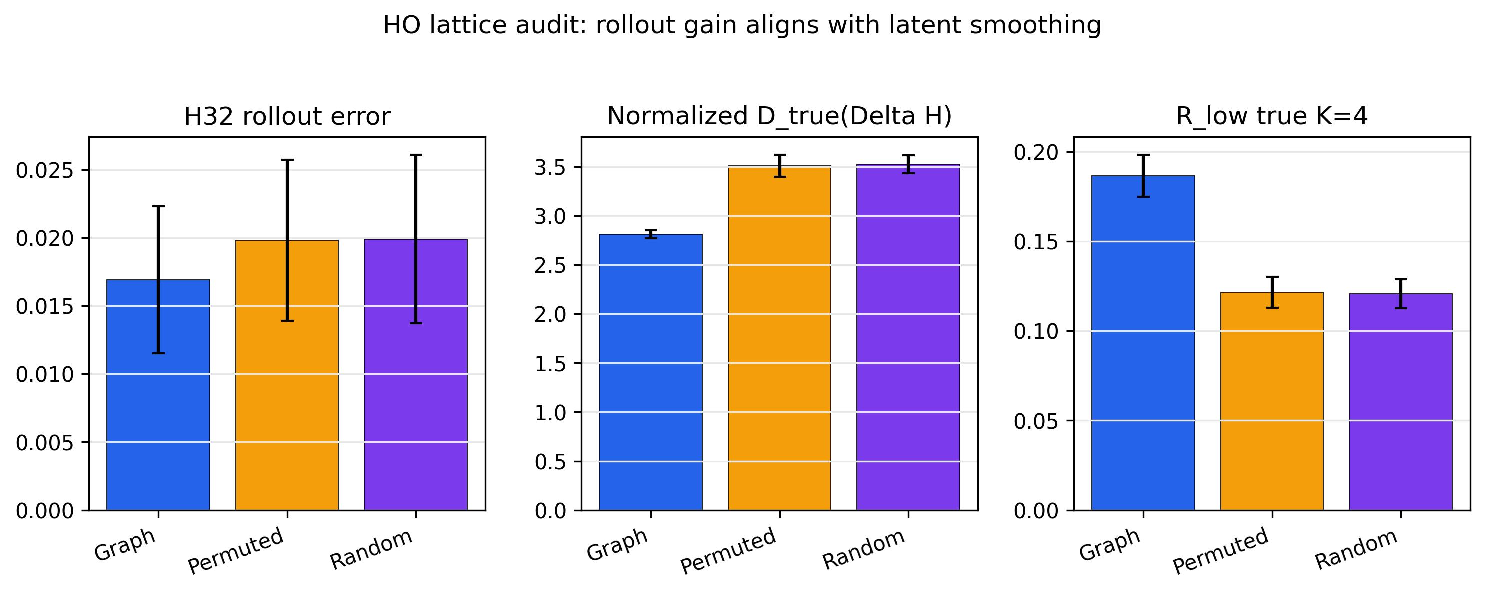
\includegraphics[width=0.85\linewidth]{figures/fig6_latent_audit_positive_case.pdf}
\caption{HO lattice audit: controlled audit-positive case. The 
candidate-graph latent temporal deltas are smoother and more 
low-frequency in the candidate-graph basis than the SMPG and 
random-graph controls. Rollout confidence intervals overlap across 
the three arms; the audit-positive classification rests on the 
agreement between rollout point-estimate ordering and latent 
audit-metric separation.}
\label{fig:ho-audit}
\end{figure}

\subsection{Generic regularization across synthetic and molecular dynamics}
\label{sec:generic-reg}

Eight cells form the generic-regularization block: three N-body 
standard cells at distance-$k$ connectivities $k=4$, $8$, $12$, and 
five rMD17 molecules that provide 3-seed historical Cycle-2 corroborating evidence without a calibrated temporal-smoothing arm.

\paragraph{N-body distance-\(k\) standard cells}
Figure~\ref{fig:nbody-standard} shows the standard-budget rollout for 
the three N-body cells. In all three, the candidate graph substantially 
improves rollout error over no-prior training. At H32, the candidate 
graph achieves mean \(\pm\) SD = \(0.064 \pm 0.032\); 95\% CI \([0.0242,0.1041]\) ($k$=4), mean \(\pm\) SD = \(0.081 \pm 0.033\); 95\% CI \([0.0402,0.1226]\) ($k$=8), and 
mean \(\pm\) SD = \(0.077 \pm 0.031\); 95\% CI \([0.0386,0.1158]\) ($k$=12), versus no-prior baselines of mean \(\pm\) SD = \(0.151 \pm 0.013\); 95\% CI \([0.1346,0.1667]\), 
mean \(\pm\) SD = \(0.152 \pm 0.012\); 95\% CI \([0.1379,0.1665]\), and mean \(\pm\) SD = \(0.144 \pm 0.012\); 95\% CI \([0.1293,0.1593]\), respectively. SEM-normalized improvements against 
the no-prior baseline are 6.01, 4.77, and 4.82 with non-overlapping CIs 
in all three cases. Against the SMPG control, however, SEM-normalized improvements 
fall to 0.54, $-0.37$, 0.91 with confidence-interval overlap in every 
cell, and against calibrated temporal smoothing they fall to 0.14, 
$-0.80$, $-1.27$ with overlap. Under the operational CI criterion, 
the candidate graph is not statistically separable from the SMPG 
control in any of the three connectivities. We therefore attribute 
the graph-vs-none improvement to generic regularization rather than 
to identifiable distance-kNN topology.

\begin{figure}[!htbp]
\centering
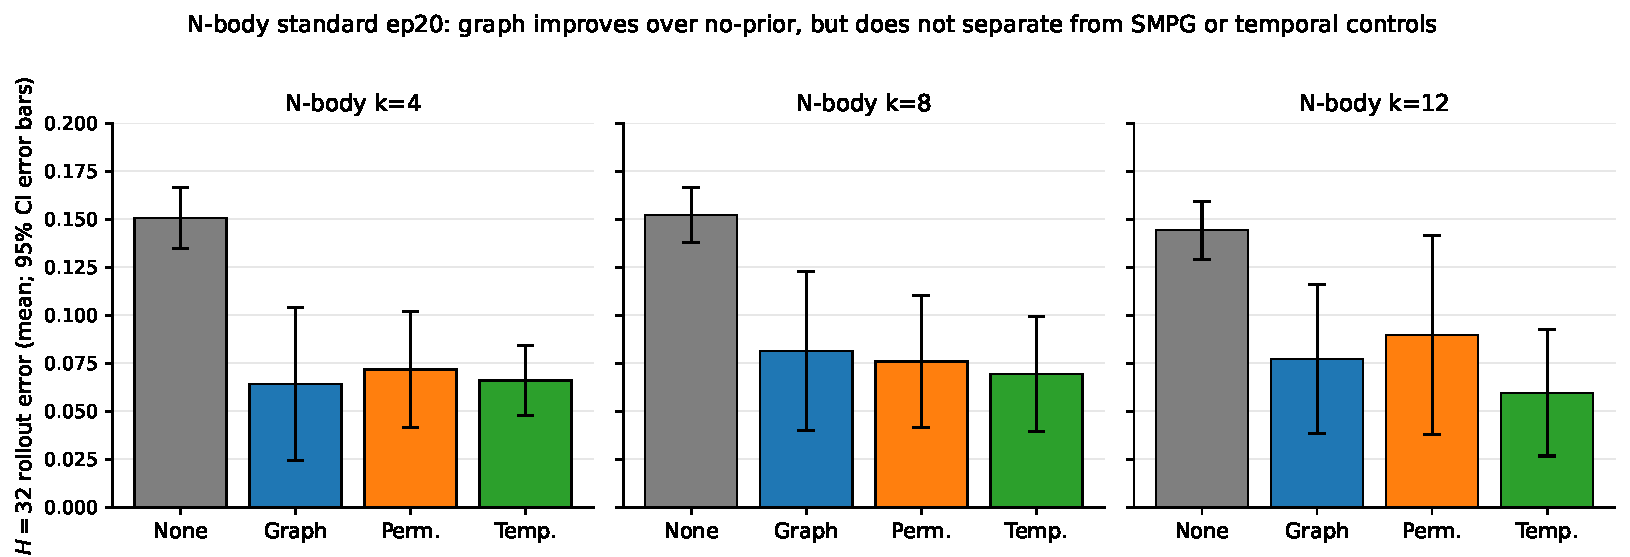
\includegraphics[width=0.95\linewidth]{figures/fig_nbody_standard_3panel.pdf}
\caption{N-body standard-budget rollout (20 epochs, 5 seeds, $H{=}32$). In all three connectivities ($k{=}4, 8, 12$) the candidate distance-kNN graph (Graph) substantially reduces rollout error against the no-prior baseline (None), but the spectrum-matched permuted graph control (Perm.) and calibrated temporal smoothing (Temp.) achieve comparable or slightly better mean rollout. Error bars are 95\% confidence intervals (t-distribution, df=4). Under the operational non-overlapping CI criterion, the candidate graph is not statistically separable from either control in any of the three cells.}
\label{fig:nbody-standard}
\end{figure}

\paragraph{rMD17 molecular-dynamics cells}
Five rMD17 molecules provide 3-seed historical Cycle-2 corroborating evidence without a calibrated temporal-smoothing arm and show the same pattern. In all five molecules, the node-wise 
graph prior has positive mean-level and SEM-normalized graph-vs-none utility: 
SEM-normalized improvements against the no-prior baseline range from 2.36 (toluene) 
to 8.37 (aspirin), spanning the same magnitude regime as N-body. 
Because \(n=3\), however, the recomputed 95\% \(t\)-intervals are wide and graph-vs-none CIs overlap in all five rMD17 molecules; we therefore do not treat these rows as strict CI-separated graph-vs-none positives. In zero of the five molecules does the candidate graph 
achieve non-overlapping CIs against the SMPG control or against the 
random-graph control. In three molecules (ethanol, malonaldehyde, 
toluene), permuted or random controls match or slightly outperform 
the candidate molecular cutoff graph at H32 (e.g., ethanol: graph 
mean \(\pm\) SD = \(0.0449 \pm 0.0036\); 95\% CI \([0.0360,0.0538]\) versus permuted mean \(\pm\) SD = \(0.0388 \pm 0.0081\); 95\% CI \([0.0187,0.0589]\); SEM-normalized improvement against 
SMPG = $-2.94$, with overlapping CIs). Because these rMD17 results 
are 3-seed historical Cycle-2 corroborating evidence without a calibrated temporal-smoothing arm, 
we use them as cross-domain corroborating practical evidence rather than as 
the sole basis for the attribution rule. They extend the 
generic-regularization classification from synthetic N-body data to 
real molecular dynamics across five distinct organic molecules.

\begin{figure}[!htbp]
\centering
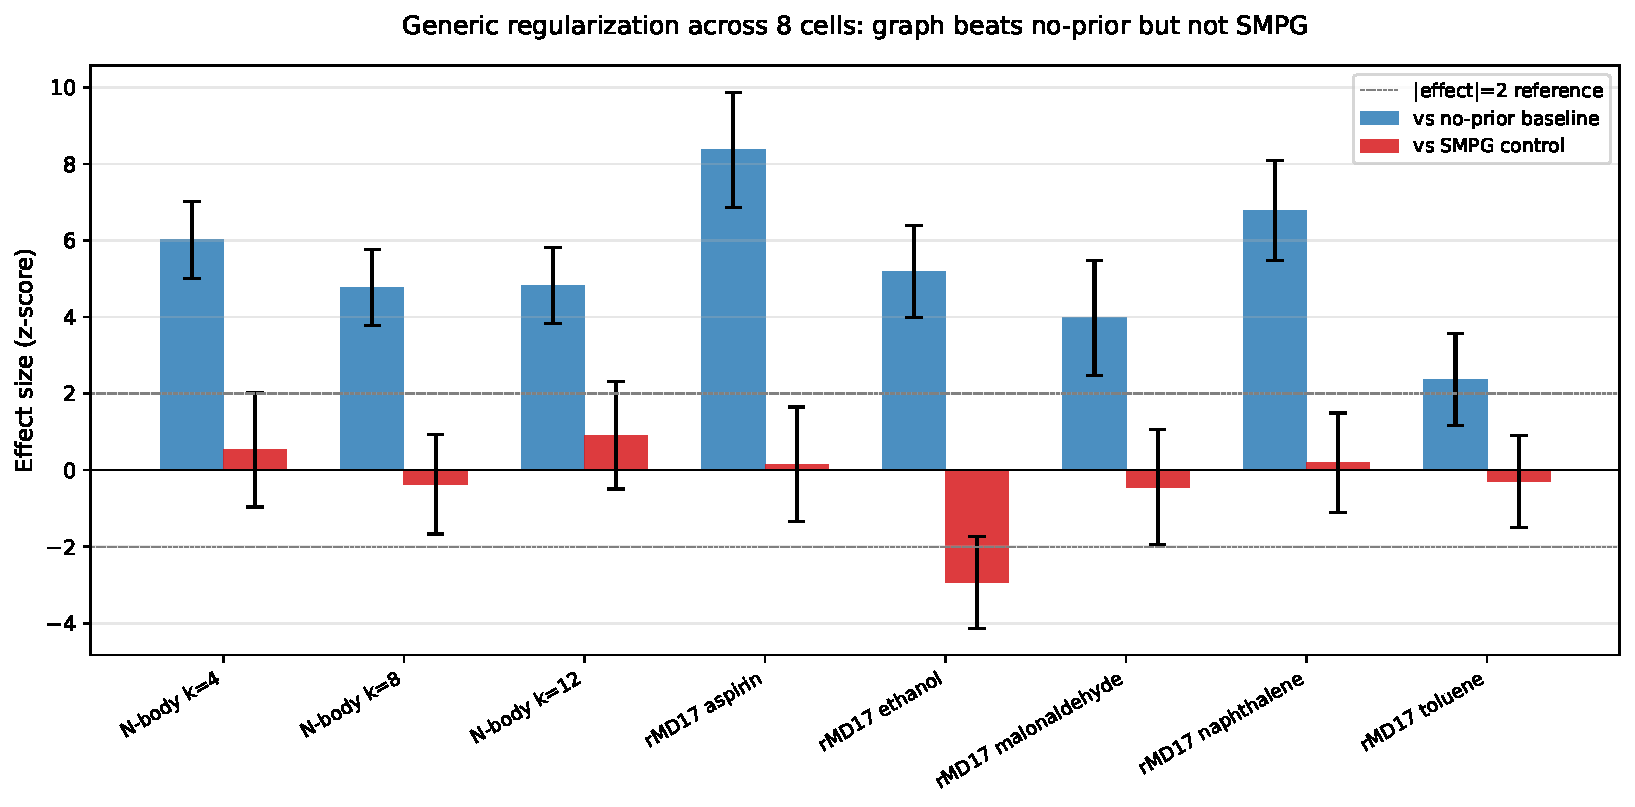
\includegraphics[width=0.95\linewidth]{figures/fig_generic_regularization_8cells.pdf}
\caption{Generic-regularization cells: SEM-normalized diagnostic improvements against the no-prior baseline (left bars) versus against the SMPG control (right bars), with 95\% confidence intervals. Across these eight cells, the graph arm shows positive graph-vs-none SEM-normalized utility, but the improvement does not separate from the SMPG control under the operational confidence-interval criterion. The rMD17 rows are 3-seed historical corroborating evidence and are interpreted as practical graph-vs-none gains rather than strict CI-separated positives.}
\label{fig:generic-reg}
\end{figure}

\subsection{No-effect cells}
\label{sec:no-effect}

Four cells show no meaningful candidate-graph effect at standard 
budget. Spring-mass lattice has graph H32 mean \(\pm\) SD = \(0.0800 \pm 0.0379\); 95\% CI \([0.0329,0.1270]\) versus 
no-prior mean \(\pm\) SD = \(0.0815 \pm 0.0136\); 95\% CI \([0.0646,0.0983]\) (SEM-normalized improvement 0.09, CI overlap). Graph-wave lattice 
has graph mean \(\pm\) SD = \(0.0782 \pm 0.0324\); 95\% CI \([0.0380,0.1185]\) versus none mean \(\pm\) SD = \(0.0833 \pm 0.0249\); 95\% CI \([0.0524,0.1143]\) (SEM-normalized improvement 0.35, 
overlap). The METR-LA correlation\_topk candidate graph has graph mean \(\pm\) SD = \(0.5243 \pm 0.2845\); 95\% CI \([-0.1826,1.2312]\) versus 
none mean \(\pm\) SD = \(0.4034 \pm 0.0609\); 95\% CI \([0.2521,0.5547]\) (SEM-normalized improvement $-0.74$; the tested correlation-derived candidate graph performs 
worse than no-prior on average, although CIs overlap). Its negative lower CI endpoint reflects a symmetric \(t\)-interval in a low-seed high-variance case and is not a physical lower bound on rollout error. This does not rule out official road adjacency, road-distance graphs, or learned traffic graphs. The graph-heat legacy single-seed cautionary cell is retained in the 
no-effect block, although it is not part of the multiseed subset: 
graph H32 = 0.6902 versus none = 0.6036, so the candidate graph 
performs worse under the tested model condition. It illustrates prior-form mismatch and is not replicated statistical evidence, so it should not be weighted equally with multiseed cells. The protocol's 
output for these cells is "do not carry the candidate graph forward 
in this model condition", which we treat as the appropriate honest 
recommendation.

\subsection{Methodological cross-validation}
\label{sec:cross-val}

As representative methodological cross-checks, we run node-order and 
transition-design diagnostics in selected regimes.

\paragraph{Node-order sanity check}
In spring-mass and N-body $k$=4, we run a node-order sanity check 
that probes whether the model's prediction pathway is sensitive to 
graph--data alignment. Three conditions are compared: (A) baseline 
(data and graph both unpermuted), (B) data and graph permuted 
consistently with the same permutation (permutation-equivariance 
check), and (C) data permuted while the candidate graph is left 
unchanged (alignment-break stress). In spring-mass, the H32 values 
are mean \(\pm\) SD = \(0.62 \pm 0.17\) for A, mean \(\pm\) SD = \(0.62 \pm 0.17\) for B, and mean \(\pm\) SD = \(0.74 \pm 0.35\) for C. The B = A 
equality confirms permutation equivariance; the C value is only 
$\sim 19\%$ worse than A despite breaking graph--data alignment, 
indicating that the prediction pathway weakly utilizes the candidate 
graph in this model condition. This yields a warning-level diagnostic rather than a pass. The same 
warning-level diagnostic is observed on N-body \(k=4\). This independent diagnostic is 
consistent with the generic-regularization classification: the model 
condition does not strongly exploit topology, regardless of prior 
strength.

\paragraph{Transition-architecture redesign}
\label{sec:transition-control}
As a robustness probe, we also tested whether the 
generic-regularization pattern was an artifact of the pooled-latent 
transition design. Replacing the transition with a graph-aware 
SAGEConv-plus-residual-MLP module stabilized by LayerNorm did not 
rescue topology attribution: spring-mass remained no-effect (SEM-normalized improvement 
against SMPG = 0.005), and N-body $k$=4 remained generic 
regularization (SEM-normalized improvement against no-prior = 3.79; SEM-normalized improvement against SMPG 
= 0.08, CI overlap). The node-order sanity warning-level diagnostic also persisted. 
We therefore treat generic-regularization dominance as a 
model-condition finding rather than a trivial artifact of the 
original transition head.

\subsection{Summary}
\label{sec:results-summary}

Across 13 measurement cells of heterogeneous evidential strength, the 
protocol identifies 1 controlled audit-positive / topology-aligned 
support cell, 0 topology-specific rollout-support cells, 8 
generic-regularization cells, and 4 no-effect cells. The 
generic-regularization cells comprise three N-body standard cells plus 
five rMD17 molecules that provide 3-seed historical Cycle-2 
corroborating evidence without a calibrated temporal-smoothing arm. The 
graph-heat legacy single-seed cautionary cell is retained as a 
no-effect cell, not as replicated statistical evidence. Without SMPG controls, and without calibrated 
temporal-smoothing controls where available, the eight 
generic-regularization cells would have appeared as 
graph-versus-no-prior successes; the protocol redirects this finding 
into the appropriate attribution class. We discuss the implications 
in Section~\ref{sec:discussion}.

\begin{table}[!htbp]
\centering
\footnotesize
\setlength{\tabcolsep}{4pt}
\renewcommand{\arraystretch}{1.08}
\caption{Compact SEM-normalized improvement and attribution summary. Standard rollout cells use H32 rollout confidence intervals for strict positives and control separation; HO is the controlled audit-positive exception.}
\label{tab:sem-summary}
\resizebox{\textwidth}{!}{%
\begin{tabular}{p{0.16\textwidth}p{0.16\textwidth}p{0.24\textwidth}p{0.30\textwidth}p{0.18\textwidth}}
\toprule
block & cells & evidence against no-prior & evidence against SMPG/random/temporal controls & attribution class \\
\midrule
HO audit & 1 controlled audit cell & No no-prior arm in the audit table. & Rollout point estimates favor graph, but graph/SMPG/random rollout CIs overlap; \(D_{\mathrm{true}}\) and \(R_{\mathrm{low}}\) separate in the expected direction. & controlled audit-positive / topology-aligned support \\
Topology-specific rollout support & 0 standard rollout cells & No current standard rollout cell both strictly improves over no-prior and separates from topology-breaking controls. & Carry any future rollout-only topology-specific positive to audit if latent artifacts are available. & topology-specific rollout support (0 cells) \\
N-body standard & \(k=4,8,12\) & Graph beats no-prior in all three cells; SEM-normalized improvements vs none are 6.014, 4.768, and 4.824 with non-overlapping CIs. & SEM-normalized improvements vs SMPG range from \(-0.370\) to 0.906 with CI overlap; calibrated temporal controls also overlap. & generic regularization \\
rMD17 molecules & aspirin, ethanol, malonaldehyde, naphthalene, toluene & 3-seed historical Cycle-2 corroborating evidence without a calibrated temporal-smoothing arm; 5/5 molecules show mean-level graph-vs-none utility, with SEM-normalized improvements vs none from 2.359 to 8.367, but low-seed \(t\)-CIs overlap. & 0/5 separate from SMPG or random controls; SEM-normalized improvements vs SMPG range from \(-2.935\) to 0.191 with CI overlap. & generic regularization \\
No-effect cells & spring-mass, graph-wave, METR-LA correlation\_topk candidate graph, graph-heat legacy single-seed cautionary cell & Graph does not clear the no-prior evidence standard, or is worse on average, under the tested model condition. & Controls do not support carrying the candidate graph forward; graph-heat legacy single-seed cautionary cell is diagnostic, not replicated statistical evidence. & no effect \\
\bottomrule
\end{tabular}
}
\noindent\emph{Note.} HO audit SEM-normalized improvements are not interpreted as rollout CI separation; rollout CIs overlap across graph, SMPG, and random controls. Classification rests on graph-favored rollout point-estimate ordering plus separated latent audit metrics. rMD17 rows are 3-seed historical Cycle-2 corroborating evidence without a calibrated temporal-smoothing arm. The graph-heat legacy single-seed cautionary cell is retained as diagnostic no-effect evidence and should not be weighted equally with multiseed cells. The METR-LA row uses a correlation-derived \path{correlation_topk} candidate graph, not official road adjacency, road-distance graphs, or learned traffic graphs. Values in prose are reported as mean \(\pm\) SD unless a 95\% CI is explicitly bracketed. Full case-level SEM-normalized rows are provided in \hyperref[app:traceability]{Appendix~D}.
\end{table}

\FloatBarrier

\section{Discussion}
\label{sec:discussion}

The main contribution of the manuscript is methodological. It 
provides a principled way to decide, under a fixed model condition, 
whether a graph-prior gain supports candidate topology, generic 
regularization, topology-specific rollout support, or no meaningful 
graph effect. In that sense, the 
protocol addresses a recurring problem in computational science: 
prior choice is consequential, but prior interpretation is easy to 
overstate.

The reported cases sharpen the distinction between predictive 
utility and topology-specific attribution. A candidate graph 
beating the no-prior baseline can be useful, but it has not yet 
shown that node-label structure matters. Across 13 measurement 
cells of heterogeneous evidential strength, including 12 replicated 
cells and one graph-heat legacy single-seed cautionary cell, the 
protocol identifies 1 controlled audit-positive / topology-aligned 
support cell, 0 topology-specific rollout-support cells, 8 
generic-regularization cells, and 4 no-effect cells. The 
generic-regularization block comprises three N-body standard cells and 
five rMD17 molecules that provide 3-seed historical Cycle-2 
corroborating evidence without a calibrated temporal-smoothing arm. 
The dominant pattern is generic regularization rather than 
topology-aligned support: in the eight generic-regularization cells, 
SEM-normalized improvements against the no-prior baseline range from 
2.4 to 8.4, but SEM-normalized improvements against 
the SMPG control range from $-2.9$ to 0.9 with confidence-interval 
overlap in every cell. Without SMPG controls, and without calibrated 
temporal-smoothing controls where available, these eight cells would 
have been over-attributed as graph-versus-no-prior successes; 
the protocol redirects them into the appropriate attribution class.

Several model-condition observations emerge from this evidence. 
First, the prediction pathway in our tested architecture weakly 
exploits topology even when the candidate graph is structurally 
plausible. The node-order sanity check provides an independent 
diagnostic of this insensitivity: in spring-mass, the alignment-break 
stress is only \(\sim 19\%\) worse than baseline, and N-body \(k=4\) 
produces the same warning-level diagnostic. Second, the 
generic-regularization classification is not a trivial artifact of 
the pooled-latent transition design: replacing the transition with a 
graph-aware SAGEConv-plus-residual-MLP module did not rescue topology 
attribution. We therefore treat generic-regularization dominance as 
a model-condition finding rather than a purely architectural failure.

The HO audit deserves special discussion. It is the only cell in 
our evidence where rollout point-estimate ordering and audit-mode 
latent metrics agree in the direction predicted by topology-aligned 
learning. Importantly, even here the rollout confidence intervals 
overlap; the audit-positive classification rests on the agreement 
between rollout ordering and latent-space audit metrics rather than 
on rollout CI separation. This is a deliberately conservative 
operational standard. The HO setting is also the only cell where 
the candidate graph corresponds exactly to the physical Laplacian, 
making it a controlled best case rather than a topology-discovery 
result. The latent audit metrics are not an independent proof that the 
learned dynamics recovered the graph; they test whether the trained 
latent trajectories exhibit the graph-basis behavior that the prior is 
intended to encourage. Their evidential value comes from agreement 
with graph-favored rollout point-estimate ordering against 
topology-breaking controls.

The negative cases reinforce the same operational lesson. The 
METR-LA correlation\_topk candidate graph diagnoses 
candidate-graph construction risk: the tested correlation-derived 
graph fails without ruling out official road adjacency, road-distance 
graphs, or learned traffic graphs. The graph-heat legacy single-seed 
cautionary cell diagnoses prior-form risk: even a true generator graph 
can fail when static Laplacian smoothing is mismatched to 
diffusion-like transition dynamics, but this single-seed result is 
diagnostic rather than replicated statistical evidence. Spring-mass and graph-wave show how the same 
workflow can recommend against carrying a candidate graph forward 
when it fails to clear the baseline. The value of the protocol, 
therefore, lies as much in ruling out unsupported interpretations as 
in identifying promising priors.

The practical value is attribution control: the protocol turns 
graph-prior successes, failures, and heterogeneous outcomes into 
diagnostic categories with explicit claim boundaries. Table~\ref{tab:headline} and the compact SEM-normalized summary in Table~\ref{tab:sem-summary} provide the main claim-level evidence. Full case-level traceability is provided in \hyperref[app:traceability]{Appendix~D} using the same values and classification rules.

\FloatBarrier

\section{Limitations}

The protocol is intentionally conservative. Its recommendations are model-conditioned and budget-conditioned: they apply to the tested encoder, transition model, latent dimension, prior placement, optimizer settings, prior strength, training budget, and rollout horizon. A recommendation should therefore be treated as a local computational conclusion rather than as a property of the dataset alone.

Several methodological boundaries follow from this framing. Candidate graphs in the reported regimes range from simulator-defined lattices to approximate physical constructions and data-derived correlation graphs, and those categories should not be interpreted in the same way. The spectrum-matched permuted graph control is the strongest control used here, but it does not exhaust every possible graph confound. A single SMPG draw may not exhaust topology-breaking nulls, especially for symmetry-rich graphs. Calibrated temporal smoothing is required for fair graph-versus-temporal comparison. Raw-coordinate diagnostics such as \(D_L(\Delta X)\) can be useful supporting probes, but because the prior acts on learned latents, they are not sufficient decision rules.

A further limitation is that audit mode depends on checkpointed latent traces or saved latent artifacts. Where those artifacts are missing, mechanism claims must remain limited. Additional prior families can be added through the same adapter interface, but they are outside the current evidence. Finally, the benchmark spans representative node-wise physical/scientific dynamics regimes rather than the whole space of scientific prediction problems, so the strongest claims are local attribution statements under the tested model condition.

Table~\ref{tab:limitations-boundaries} consolidates these boundaries.

\begingroup
\footnotesize
\setlength{\tabcolsep}{4pt}
\begin{longtable}{>{\raggedright\arraybackslash}p{0.18\textwidth}>{\raggedright\arraybackslash}p{0.44\textwidth}>{\raggedright\arraybackslash}p{0.28\textwidth}}
\caption{Limitations and claim boundaries}\label{tab:limitations-boundaries}\\
\toprule
\textbf{limitation or boundary} & \textbf{boundary statement} & \textbf{implication} \\
\midrule
\endfirsthead
\toprule
\textbf{limitation or boundary} & \textbf{boundary statement} & \textbf{implication} \\
\midrule
\endhead
\midrule
\multicolumn{3}{r}{\emph{Continued on next page}} \\
\midrule
\endfoot
\bottomrule
\endlastfoot
Model conditioning & Recommendations apply under the tested encoder, transition model, prior placement, prior strength, optimizer, training budget, and rollout horizon. & Changing the model condition requires a new preflight interpretation. \\
Budget conditioning & Short-budget gains can disappear under standard or longer training. & Initial positives should be validated before stronger claims. \\
Candidate graph ambiguity & Candidate graphs may be true, approximate, constructed, or data-derived. The METR-LA result tests a correlation-derived \path{correlation_topk} candidate graph, not official road adjacency, road-distance graphs, or learned traffic graphs. & A useful candidate graph prior does not prove physical truth, and a failed data-derived candidate does not rule out other graph constructions. \\
Control requirements & In standard rollout cells, topology-specific attribution requires separation from the spectrum-matched permuted graph control and calibrated temporal smoothing where available. & Graph versus none is insufficient for topology-specific attribution. \\
Temporal calibration & Raw temporal prior losses may be much smaller than graph-prior losses. & Temporal baselines should be calibrated before attribution. \\
Raw diagnostics & Raw-coordinate smoothness can disagree with learned latent prior utility. & Raw $D_L(\Delta X)$ should not be used as a sufficient decision rule. \\
Audit artifacts & Latent audits require saved traces or checkpoints. & Missing artifacts limit mechanism claims. \\
Benchmark scope & Regimes are representative stress tests, not exhaustive scientific prediction coverage; rMD17 is 3-seed historical Cycle-2 corroborating evidence without a calibrated temporal-smoothing arm, and the graph-heat legacy single-seed cautionary cell is not replicated statistical evidence. & Interpret conclusions as local model-conditioned attribution statements and weight evidence by replication strength. \\
Causal claims & The workflow compares predictive priors and controls. & Do not frame the result as causal discovery. \\
Prior novelty & The graph Laplacian prior is a tested prior family, not the paper's algorithmic novelty. & The contribution is the preflight protocol and attribution workflow. \\
\end{longtable}
\endgroup

\section{Conclusion}
\label{sec:conclusion}

This manuscript presents a model-conditioned attribution protocol for 
graph priors in node-wise scientific latent dynamics. By combining 
no-prior baselines, a candidate graph prior, the spectrum-matched 
permuted graph control, random-graph controls when available, 
calibrated temporal smoothing where available, and audit mode when 
latent artifacts are available, the protocol turns graph-prior gains 
into controlled attribution decisions rather than graph-versus-no-prior 
anecdotes.

Across 13 measurement cells of heterogeneous evidential strength, 
including 12 replicated cells and one graph-heat legacy single-seed 
cautionary cell, the protocol identifies 1 controlled audit-positive / 
topology-aligned support cell, 0 topology-specific rollout-support cells, 
8 generic-regularization cells, and 4 no-effect cells. The dominant 
pattern is generic regularization rather than topology-aligned support. 
Eight of the 13 cells, spanning N-body synthetic data and five rMD17 
molecules that provide 3-seed historical Cycle-2 corroborating evidence 
without a calibrated temporal-smoothing arm, show graph-vs-none utility 
or practical gain, but do not separate from the spectrum-matched 
permuted graph control under the operational confidence-interval 
criterion. The HO 
lattice audit is the single controlled audit-positive / topology-aligned 
support case, where rollout ordering and audit-mode latent metrics agree 
in the direction predicted by topology-aligned learning. The protocol 
finds zero topology-specific rollout-support cells in the current 
evidence. Four no-effect cells (spring-mass, graph-wave, the METR-LA 
correlation\_topk candidate graph, and the graph-heat legacy single-seed cautionary cell) show 
that graph priors do not always provide regularization benefit even 
under matched conditions. The main empirical lesson is negative but 
useful: in the tested model condition, most graph-prior gains are real 
predictive gains but not topology-specific gains. SMPG controls should 
be reported before graph-prior improvements are interpreted as 
topology-specific.

The contribution is therefore a practical workflow for prior 
selection and interpretation under fixed model conditions. The 
protocol's primary value is attribution control: it converts ambiguous 
"graph-vs-none" gains into structured operational outcomes that can 
guide subsequent computational decisions.

\section*{Data and Code Availability}
This manuscript reports completed runs from the associated project repository. The preflight tool is implemented as an adapter-based script in which dataset-specific adapters provide trajectories and candidate graph information, while the shared routine writes \texttt{run\_config.json}, \texttt{summary.csv}, and \texttt{preflight\_report.md} as standardized run artifacts. Code and manuscript assets will be made available through an anonymized repository during review and through a public archival repository upon acceptance.

\FloatBarrier

\appendix

\section{Protocol details and operating modes}

The protocol is best understood as a sequence of increasingly demanding questions. The first question is whether any prior helps over no-prior training. The second is whether the gain survives the spectrum-matched permuted graph (SMPG) control and calibrated temporal smoothing where available. Audit mode, when checkpointed latent traces are available, asks whether predictive gains coincide with latent behavior consistent with the candidate graph. The strongest label therefore requires agreement across utility, control comparisons, and latent-space evidence.

The attribution outcomes in Table~\ref{tab:protocol-labels} should be interpreted as report-level decisions rather than as permanent properties of a dataset. They are intentionally conservative: controlled audit-positive / topology-aligned support is reserved for the HO audit because rollout ordering agrees with separated latent audit metrics; topology-specific rollout support is retained as a zero-count rollout-only outcome for future cells that separate from topology-breaking controls before audit; generic regularization marks graph-vs-none gains that do not separate from topology-breaking controls; and no effect recommends against carrying the tested candidate graph forward under the current model condition.

\section{Benchmark regimes and dataset-adapter notes}

The benchmark set mixes graphs with different provenance. HO, spring-mass, graph-wave, and the graph-heat legacy single-seed cautionary cell use true or simulator-defined lattices. N-body uses an approximate distance-kNN graph. The rMD17 summaries are 3-seed historical Cycle-2 corroborating evidence without a calibrated temporal-smoothing arm and use molecular cutoff graphs. METR-LA uses a correlation-derived \path{correlation_topk} sensor graph rather than official road adjacency. Auxiliary constructed spectral stress tests are excluded from the 13-cell headline count. This variation is intentional because candidate graph provenance is part of the interpretation boundary addressed by the preflight protocol.

\section{Prior families and calibration formulas}

The graph Laplacian prior on learned node-wise latent states is

\begin{equation}
R_G(H;L)=\mathrm{Tr}(H^\top L H)
\end{equation}

The spectrum-matched permuted graph control is

\begin{equation}
L_{\mathrm{perm}} = P^T L P,
\end{equation}

where $P$ is a permutation matrix. This preserves Laplacian eigenvalues while disrupting node-label semantics.

The graph-free temporal smoothness prior is

\begin{equation}
R_T(H_{1:T})=\sum_t \lVert H_{t+1}-H_t \rVert_F^2
\end{equation}

For calibrated prior-strength matching, let $\alpha_G$ be the graph-prior weight, and let $R_G^0$ and $R_T^0$ denote initial graph and temporal prior losses under the same calibration pass. The calibrated temporal weight is

\begin{equation}
\alpha_T = \frac{\alpha_G R_G^0}{R_T^0+\varepsilon}
\end{equation}

so that

\begin{equation}
\alpha_T R_T^0 \approx \alpha_G R_G^0
\end{equation}

\section{Claim traceability and supporting evidence}
\label{app:traceability}

This appendix provides a compact traceability table linking each major manuscript claim to the supporting experiment summaries, key numerical evidence, and interpretation caveats.

\begingroup
\scriptsize
\setlength{\tabcolsep}{3pt}
\begin{longtable}{>{\raggedright\arraybackslash}p{0.22\textwidth}>{\raggedright\arraybackslash}p{0.18\textwidth}>{\raggedright\arraybackslash}p{0.21\textwidth}>{\raggedright\arraybackslash}p{0.17\textwidth}>{\raggedright\arraybackslash}p{0.12\textwidth}}
\caption{Claim traceability and supporting evidence}\label{tab:evidence-map}\\
\toprule
\textbf{claim} & \textbf{supporting evidence} & \textbf{current values} & \textbf{boundary} & \textbf{appears in} \\
\midrule
\endfirsthead
\toprule
\textbf{claim} & \textbf{supporting evidence} & \textbf{current values} & \textbf{boundary} & \textbf{appears in} \\
\midrule
\endhead
\midrule
\multicolumn{5}{r}{\emph{Continued on next page}} \\
\midrule
\endfoot
\bottomrule
\endlastfoot
The protocol is an attribution workflow, not a SOTA benchmark. & \path{paper/tables/headline_attribution_table.md}; \path{paper/tables/master_multiseed_summary.md} & Model condition includes encoder, transition model, latent dimension, prior placement, prior strength, training budget, and rollout horizon. & The contribution is prior selection and interpretation under a fixed model condition, not a new graph prior or universal predictor. & Sections 1--5 \\
SMPG controls prevent over-attribution. & \path{paper/tables/effect_size_unified.md}; \path{analysis_out/effect_size_analysis.md} & Across the eight generic-regularization cells, SEM-normalized improvements vs none are 2.359--8.367, while SEM-normalized improvements vs SMPG are \(-2.935\)--0.906 with CI overlap in every cell. & Graph-vs-none utility does not identify candidate topology. & Tables~\ref{tab:headline}--\ref{tab:sem-summary} \\
HO is controlled audit-positive; rollout CIs overlap and audit metrics separate. & \path{paper/tables/master_multiseed_summary.md}; \path{paper/figure_data/fig6_latent_audit_positive_case.csv} & H32 graph mean \(\pm\) SD = $0.0169\pm0.0054$; 95\% CI $[0.0102,0.0236]$, SMPG mean \(\pm\) SD = $0.0198\pm0.0059$; 95\% CI $[0.0125,0.0271]$, random mean \(\pm\) SD = $0.0199\pm0.0062$; 95\% CI $[0.0122,0.0275]$; \(D_{\mathrm{true}}\) graph $2.81$ vs SMPG $3.51$; \(R_{\mathrm{low}}\) graph $0.187$ vs SMPG $0.122$. & Controlled support, not topology discovery; classification is not based on rollout CI separation. & Section~\ref{sec:ho-audit} \\
N-body \(k=4,8,12\) are generic regularization. & \path{paper/tables/master_multiseed_summary.md}; \path{paper/tables/effect_size_unified.md} & SEM-normalized improvements vs none are 6.014, 4.768, 4.824; values vs SMPG are 0.535, \(-0.370\), 0.906 with overlap; temporal controls overlap. & Approximate distance-kNN graph utility is not topology-specific attribution under this model condition. & Section~\ref{sec:generic-reg} \\
rMD17 five molecules corroborate generic regularization. & \path{paper/tables/master_multiseed_summary.md}; \path{analysis_out/rmd17_historical_summary.md} & 3-seed historical Cycle-2 corroborating evidence without a calibrated temporal-smoothing arm; 5/5 molecules show mean-level graph-vs-none utility, but low-seed \(t\)-CIs overlap; 0/5 separate from SMPG/random controls. SEM-normalized improvements vs SMPG are 0.147, \(-2.935\), \(-0.445\), 0.191, \(-0.289\). & Used as corroborating cross-domain practical evidence, not the sole basis for the attribution rule. & Section~\ref{sec:generic-reg} \\
Spring-mass, graph-wave, METR-LA correlation\_topk candidate graph, and graph-heat legacy single-seed cautionary cell are no-effect cells. & \path{paper/tables/master_multiseed_summary.md}; \path{paper/tables/effect_size_unified.md} & Spring-mass SEM-normalized improvement vs none 0.088; graph-wave 0.352; METR-LA correlation\_topk candidate graph \(-0.736\); graph-heat legacy single-seed cautionary cell graph H32 $0.6902$ vs none $0.6036$. & METR-LA uses a correlation-derived candidate graph and does not rule out official road adjacency, road-distance graphs, or learned traffic graphs; graph-heat legacy single-seed cautionary cell is diagnostic, not replicated statistical evidence. & Section~\ref{sec:no-effect} \\
Node-order sanity indicates weak graph utilization. & \path{analysis_out/NODE_ORDER_SANITY_REPORT.md}; \path{paper/tables/node_order_sanity_summary.md} & Spring-mass H32 mean \(\pm\) SD = $0.62\pm0.17$ for A, mean \(\pm\) SD = $0.62\pm0.17$ for B, and mean \(\pm\) SD = $0.74\pm0.35$ for C; N-body \(k=4\) gives the same warning-level diagnostic. & Diagnostic evidence supports weak topology use, but it is not itself an attribution class. & Section~\ref{sec:cross-val} \\
Graph-aware transition redesign did not rescue topology attribution. & \path{analysis_out/transition_redesign_proposal.md}; \path{analysis_out/transition_layernorm_validation.md}; \path{analysis_out/transition_instability_diagnosis.md} & SAGEConv-plus-residual-MLP with LayerNorm leaves spring-mass no-effect (SEM-normalized improvement vs SMPG $0.005$) and N-body \(k=4\) generic regularization (SEM-normalized improvement vs none $3.79$, vs SMPG $0.08$, CI overlap). & This is a model-condition robustness probe, not a universal architecture comparison. & Section~\ref{sec:transition-control} \\
\end{longtable}
\endgroup

\subsection*{Case-level SEM-normalized rows}

\begingroup
\scriptsize
\setlength{\tabcolsep}{3pt}
\renewcommand{\arraystretch}{1.05}
\begin{longtable}{>{\raggedright\arraybackslash}p{0.18\textwidth}>{\raggedright\arraybackslash}p{0.06\textwidth}>{\raggedright\arraybackslash}p{0.09\textwidth}>{\raggedright\arraybackslash}p{0.10\textwidth}>{\raggedright\arraybackslash}p{0.10\textwidth}>{\raggedright\arraybackslash}p{0.20\textwidth}>{\raggedright\arraybackslash}p{0.11\textwidth}}
\caption{Appendix case-level SEM-normalized rows consistent with Tables~\ref{tab:headline}--\ref{tab:sem-summary}}\label{tab:app-sem-normalized}\\
\toprule
\textbf{cell} & \textbf{seeds} & \textbf{graph H32} & \textbf{SEM-norm. vs none} & \textbf{SEM-norm. vs SMPG} & \textbf{control status} & \textbf{class} \\
\midrule
\endfirsthead
\toprule
\textbf{cell} & \textbf{seeds} & \textbf{graph H32} & \textbf{SEM-norm. vs none} & \textbf{SEM-norm. vs SMPG} & \textbf{control status} & \textbf{class} \\
\midrule
\endhead
\midrule
\multicolumn{7}{r}{\emph{Continued on next page}} \\
\midrule
\endfoot
\bottomrule
\endlastfoot
HO lattice audit & 5 & $0.0169$ & N/A & $3.083$ audit & Rollout CIs overlap; audit metrics separate vs SMPG/random. & controlled audit-positive \\
N-body \(k=4\) standard & 5 & $0.0641$ & $6.014$ & $0.535$ & CI-separated vs none; overlap vs SMPG and temporal. & generic regularization \\
N-body \(k=8\) standard & 5 & $0.0814$ & $4.768$ & $-0.370$ & CI-separated vs none; overlap vs SMPG and temporal. & generic regularization \\
N-body \(k=12\) standard & 5 & $0.0772$ & $4.824$ & $0.906$ & CI-separated vs none; overlap vs SMPG and temporal. & generic regularization \\
rMD17 aspirin & 3 & $0.0306$ & $8.367$ & $0.147$ & Mean-level graph-vs-none utility; low-seed \(t\)-CIs overlap; overlap vs SMPG/random. & generic regularization \\
rMD17 ethanol & 3 & $0.0449$ & $5.196$ & $-2.935$ & Mean-level graph-vs-none utility; low-seed \(t\)-CIs overlap; overlap vs SMPG/random. & generic regularization \\
rMD17 malonaldehyde & 3 & $0.0346$ & $3.979$ & $-0.445$ & Mean-level graph-vs-none utility; low-seed \(t\)-CIs overlap; overlap vs SMPG/random. & generic regularization \\
rMD17 naphthalene & 3 & $0.0210$ & $6.785$ & $0.191$ & Mean-level graph-vs-none utility; low-seed \(t\)-CIs overlap; overlap vs SMPG/random. & generic regularization \\
rMD17 toluene & 3 & $0.0323$ & $2.359$ & $-0.289$ & Mean-level graph-vs-none utility; low-seed \(t\)-CIs overlap; overlap vs SMPG/random. & generic regularization \\
Graph-heat legacy single-seed cautionary cell & 1 & $0.6902$ & N/A & N/A & Single-seed caution; graph worse than no-prior; not replicated statistical evidence. & no effect \\
Graph-wave standard & 5 & $0.0782$ & $0.352$ & $-0.469$ & Overlap vs none, SMPG, and temporal. & no effect \\
METR-LA correlation\_topk candidate graph & 3 & $0.5243$ & $-0.736$ & $-0.132$ & Correlation-derived graph worse than no-prior on average; CIs overlap. & no effect \\
Spring-mass standard & 5 & $0.0800$ & $0.088$ & $0.189$ & Overlap vs none, SMPG, and temporal. & no effect \\
\end{longtable}
\endgroup

\noindent\emph{Note.} Values in prose are reported as mean \(\pm\) SD unless a 95\% CI is explicitly bracketed. Figure error bars use 95\% CIs where stated. The SEM-normalized diagnostic is not a formal hypothesis-test \(z\) statistic or Cohen's \(d\).

\section{Reproducibility and control availability}
\label{app:reproducibility}
\label{app:reproducibility-tables}

Tables~\ref{tab:model-condition} and \ref{tab:control-availability} summarize the fixed model conditions and control availability recorded in the run artifacts. When a field is not present in the available artifact, the table states this explicitly rather than inferring a value.

\begingroup
\scriptsize
\setlength{\tabcolsep}{3pt}
\renewcommand{\arraystretch}{1.08}
\begin{longtable}{>{\raggedright\arraybackslash}p{0.16\textwidth}>{\raggedright\arraybackslash}p{0.20\textwidth}>{\raggedright\arraybackslash}p{0.18\textwidth}>{\raggedright\arraybackslash}p{0.18\textwidth}>{\raggedright\arraybackslash}p{0.20\textwidth}}
\caption{Fixed model condition used in reported preflight runs}\label{tab:model-condition}\\
\toprule
\textbf{reported block} & \textbf{encoder / transition / latent} & \textbf{prior placement and weight} & \textbf{optimization and budget} & \textbf{artifact notes} \\
\midrule
\endfirsthead
\toprule
\textbf{reported block} & \textbf{encoder / transition / latent} & \textbf{prior placement and weight} & \textbf{optimization and budget} & \textbf{artifact notes} \\
\midrule
\endhead
\midrule
\multicolumn{5}{r}{\emph{Continued on next page}} \\
\midrule
\endfoot
\bottomrule
\endlastfoot
N-body \(k=4,8,12\), spring-mass, graph-wave standard cells & \texttt{gnn\_node} encoder; node-wise GraphSAGE encoder layers and pooled-latent MLP transition; latent/node dimension 16, hidden dimension 64, transition hidden dimension 64. & Graph Laplacian prior on learned node-wise latents; nominal prior weight 0.1; Laplacian normalized by \(\lambda_{\max}\); calibrated temporal-smoothing arm where reported. & Adam optimizer, learning rate 0.001, batch size 32, 20 epochs, 96 train transitions, 32 eval transitions, horizons H16/H32, seeds 0--4, device \texttt{auto}. & Values from \path{analysis_out/preflight_runs/*/standard_ep20/run_config.json} and \path{scripts/graph_prior_preflight_check.py}. Exact hardware is not reported in the run artifacts. \\
METR-LA correlation\_topk candidate graph & Same \texttt{gnn\_node} / pooled-latent MLP model condition; latent/node dimension 16, hidden dimension 64, transition hidden dimension 64. & Data-derived \path{correlation_topk} candidate graph, \(k=8\); nominal prior weight 0.1; \(\lambda_{\max}\) normalization; calibrated temporal arm reported. & Adam optimizer, learning rate 0.001, batch size 32, 5 epochs, 160 train transitions, 64 eval transitions, horizons H16/H32, seeds 0--2, device \texttt{auto}. & Values from \path{analysis_out/preflight_runs/metr_la_3seed/corr_T2000_train160_ep5/run_config.json}; max timesteps 2000. \\
rMD17 Cycle-2 molecules & \texttt{gnn\_node} graph/control arms and \texttt{gnn\_node} no-prior comparator; latent/node dimension 16, hidden dimension 64, transition hidden dimension 64. & Molecular cutoff graph prior and topology-breaking graph controls; nominal prior weight 0.1. & Adam optimizer, learning rate 0.001, batch size 32, 30 epochs, 96 train transitions, 24 eval transitions, horizons H1, H2, H4, H8, H16, H32, seeds 0--2, device \texttt{auto}. & Values from \path{experiments/results/cycle2_rmd17_multimolecule/cycle2_rmd17_multimolecule_results.json}; 3-seed historical Cycle-2 corroborating evidence without a calibrated temporal-smoothing arm. \\
HO lattice audit & \texttt{gnn\_node} encoder; latent/node dimension 16, hidden dimension 64, transition hidden dimension 64; checkpointed latent traces available. & True physical lattice Laplacian or topology-breaking graph control; nominal prior weight 0.1. & Adam optimizer, learning rate 0.001, batch size 32, 30 epochs, 96 train transitions, 24 eval transitions, horizons H1, H2, H4, H8, H16, H32, seeds 0--4, device \texttt{auto}. & Values from \path{analysis_out/preflight_runs/ho_audit_5seed/cycle8_ho_audit_results.json}; no no-prior arm in the audit table. \\
Graph-heat legacy single-seed cautionary cell & Legacy single-seed row retained from \path{paper/tables/master_multiseed_summary.md}; available run-config analogue uses \texttt{gnn\_node} / pooled-latent MLP with latent/node dimension 16. & True generator graph; nominal prior weight 0.1 in available run-config analogue. & Legacy headline row is single-seed only. Available run-config analogue records Adam, learning rate 0.001, batch size 32, 5 epochs, 96 train transitions, 32 eval transitions, H16/H32, seeds 0--2. & The 13-cell headline uses the legacy single-seed aggregate because no standard-budget multiseed counterpart is present in current derived outputs. \\
\end{longtable}
\endgroup

\begingroup
\tiny
\setlength{\tabcolsep}{1pt}
\renewcommand{\arraystretch}{1.08}
\begin{longtable}{>{\raggedright\arraybackslash}p{0.17\textwidth}>{\centering\arraybackslash}p{0.035\textwidth}>{\raggedright\arraybackslash}p{0.175\textwidth}>{\centering\arraybackslash}p{0.045\textwidth}>{\centering\arraybackslash}p{0.045\textwidth}>{\centering\arraybackslash}p{0.055\textwidth}>{\centering\arraybackslash}p{0.055\textwidth}>{\centering\arraybackslash}p{0.055\textwidth}>{\centering\arraybackslash}p{0.045\textwidth}>{\centering\arraybackslash}p{0.045\textwidth}>{\centering\arraybackslash}p{0.045\textwidth}}
\caption{Regime and control availability summary}\label{tab:control-availability}\\
\toprule
\textbf{cell} & \textbf{n} & \textbf{graph provenance} & \textbf{none} & \textbf{graph} & \textbf{SMPG} & \textbf{rand.} & \textbf{temp.} & \textbf{audit} & \textbf{repl.} & \textbf{single} \\
\midrule
\endfirsthead
\toprule
\textbf{cell} & \textbf{n} & \textbf{graph provenance} & \textbf{none} & \textbf{graph} & \textbf{SMPG} & \textbf{rand.} & \textbf{temp.} & \textbf{audit} & \textbf{repl.} & \textbf{single} \\
\midrule
\endhead
\midrule
\multicolumn{11}{r}{\emph{Continued on next page}} \\
\midrule
\endfoot
\bottomrule
\endlastfoot
HO lattice audit & 5 & true simulator lattice / physical Laplacian & no & yes & yes & yes & no & yes & yes & no \\
N-body \(k=4\) standard & 5 & approximate distance-kNN graph & yes & yes & yes & no & yes & no & yes & no \\
N-body \(k=8\) standard & 5 & approximate distance-kNN graph & yes & yes & yes & no & yes & no & yes & no \\
N-body \(k=12\) standard & 5 & approximate distance-kNN graph & yes & yes & yes & no & yes & no & yes & no \\
rMD17 aspirin & 3 & molecular cutoff graph & yes & yes & yes & yes & no & no & yes & no \\
rMD17 ethanol & 3 & molecular cutoff graph & yes & yes & yes & yes & no & no & yes & no \\
rMD17 malonaldehyde & 3 & molecular cutoff graph & yes & yes & yes & yes & no & no & yes & no \\
rMD17 naphthalene & 3 & molecular cutoff graph & yes & yes & yes & yes & no & no & yes & no \\
rMD17 toluene & 3 & molecular cutoff graph & yes & yes & yes & yes & no & no & yes & no \\
Spring-mass standard & 5 & true spring lattice & yes & yes & yes & not rep. & yes & no & yes & no \\
Graph-wave standard & 5 & true wave lattice & yes & yes & yes & not rep. & yes & no & yes & no \\
METR-LA correlation\_topk candidate graph & 3 & data-derived correlation sensor graph & yes & yes & yes & not rep. & yes & no & yes & no \\
Graph-heat legacy single-seed cautionary cell & 1 & true generator graph & yes & yes & yes & not rep. & not rep. & no & no & yes \\
\end{longtable}
\endgroup

\section{Case-level H32 rollout summaries}
\label{app:case-level-rollout}
\label{app:h32-summaries}

\begingroup
\scriptsize
\setlength{\tabcolsep}{2pt}
\renewcommand{\arraystretch}{1.18}
\newcommand{\hci}[3]{#1 \(\pm\) #2; 95\% CI [#3]}
\noindent Tables~\ref{tab:h32-ho-nbody}--\ref{tab:h32-no-effect} report case-level H32 rollout summaries by prior arm. Entries use mean \(\pm\) SD; 95\% CI [lower, upper] when \(n>1\). Symmetric \(t\)-intervals are uncertainty summaries for seed means; in high-variance low-seed cells they may cross zero and should not be interpreted as physical error bounds. The graph-heat legacy single-seed cautionary cell has no confidence interval reported or interpreted.

\begin{table}[H]
\centering
\caption{Case-level H32 rollout summaries by prior arm: HO audit and N-body}\label{tab:h32-ho-nbody}
\begin{tabularx}{\textwidth}{>{\raggedright\arraybackslash}p{0.15\textwidth}>{\centering\arraybackslash}p{0.035\textwidth}>{\raggedright\arraybackslash}X>{\raggedright\arraybackslash}X>{\raggedright\arraybackslash}X>{\raggedright\arraybackslash}X>{\raggedright\arraybackslash}X>{\raggedright\arraybackslash}p{0.13\textwidth}}
\toprule
\textbf{cell} & \textbf{n} & \textbf{none} & \textbf{graph} & \textbf{SMPG} & \textbf{random} & \textbf{temporal} & \textbf{outcome} \\
\midrule
HO lattice audit & 5 & not run & \hci{0.0169}{0.0054}{0.0102, 0.0236} & \hci{0.0198}{0.0059}{0.0125, 0.0271} & \hci{0.0199}{0.0062}{0.0122, 0.0275} & not run & controlled audit-positive / topology-aligned support \\
N-body \(k=4\) & 5 & \hci{0.1507}{0.0129}{0.1346, 0.1667} & \hci{0.0641}{0.0322}{0.0242, 0.1041} & \hci{0.0718}{0.0245}{0.0414, 0.1021} & not run & \hci{0.0661}{0.0147}{0.0479, 0.0843} & generic regularization \\
N-body \(k=8\) & 5 & \hci{0.1522}{0.0115}{0.1379, 0.1665} & \hci{0.0814}{0.0332}{0.0402, 0.1226} & \hci{0.0759}{0.0276}{0.0416, 0.1102} & not run & \hci{0.0695}{0.0240}{0.0397, 0.0992} & generic regularization \\
N-body \(k=12\) & 5 & \hci{0.1443}{0.0121}{0.1293, 0.1593} & \hci{0.0772}{0.0311}{0.0386, 0.1158} & \hci{0.0898}{0.0417}{0.0380, 0.1416} & not run & \hci{0.0596}{0.0265}{0.0267, 0.0925} & generic regularization \\
\bottomrule
\end{tabularx}
\end{table}

\begin{table}[H]
\centering
\caption{Case-level H32 rollout summaries by prior arm: rMD17 molecules}\label{tab:h32-rmd17}
\begin{tabularx}{\textwidth}{>{\raggedright\arraybackslash}p{0.15\textwidth}>{\centering\arraybackslash}p{0.035\textwidth}>{\raggedright\arraybackslash}X>{\raggedright\arraybackslash}X>{\raggedright\arraybackslash}X>{\raggedright\arraybackslash}X>{\raggedright\arraybackslash}X>{\raggedright\arraybackslash}p{0.13\textwidth}}
\toprule
\textbf{cell} & \textbf{n} & \textbf{none} & \textbf{graph} & \textbf{SMPG} & \textbf{random} & \textbf{temporal} & \textbf{outcome} \\
\midrule
rMD17 aspirin & 3 & \hci{0.0934}{0.0230}{0.0363, 0.1505} & \hci{0.0306}{0.0130}{-0.0017, 0.0629} & \hci{0.0317}{0.0078}{0.0123, 0.0511} & \hci{0.0305}{0.0083}{0.0099, 0.0511} & not run & generic regularization \\
rMD17 ethanol & 3 & \hci{0.0557}{0.0163}{0.0152, 0.0962} & \hci{0.0449}{0.0036}{0.0360, 0.0538} & \hci{0.0388}{0.0081}{0.0187, 0.0589} & \hci{0.0400}{0.0040}{0.0301, 0.0499} & not run & generic regularization \\
rMD17 malonaldehyde & 3 & \hci{0.0686}{0.0189}{0.0216, 0.1156} & \hci{0.0346}{0.0148}{-0.0022, 0.0714} & \hci{0.0308}{0.0082}{0.0104, 0.0512} & \hci{0.0305}{0.0091}{0.0079, 0.0531} & not run & generic regularization \\
rMD17 naphthalene & 3 & \hci{0.0637}{0.0219}{0.0093, 0.1181} & \hci{0.0210}{0.0109}{-0.0061, 0.0481} & \hci{0.0222}{0.0125}{-0.0089, 0.0533} & \hci{0.0234}{0.0122}{-0.0069, 0.0537} & not run & generic regularization \\
rMD17 toluene & 3 & \hci{0.0609}{0.0226}{0.0048, 0.1170} & \hci{0.0323}{0.0210}{-0.0199, 0.0845} & \hci{0.0288}{0.0125}{-0.0023, 0.0599} & \hci{0.0293}{0.0136}{-0.0045, 0.0631} & not run & generic regularization \\
\bottomrule
\end{tabularx}
\end{table}

\begin{table}[H]
\centering
\caption{Case-level H32 rollout summaries by prior arm: no-effect cells}\label{tab:h32-no-effect}
\begin{tabularx}{\textwidth}{>{\raggedright\arraybackslash}p{0.15\textwidth}>{\centering\arraybackslash}p{0.035\textwidth}>{\raggedright\arraybackslash}X>{\raggedright\arraybackslash}X>{\raggedright\arraybackslash}X>{\raggedright\arraybackslash}X>{\raggedright\arraybackslash}X>{\raggedright\arraybackslash}p{0.13\textwidth}}
\toprule
\textbf{cell} & \textbf{n} & \textbf{none} & \textbf{graph} & \textbf{SMPG} & \textbf{random} & \textbf{temporal} & \textbf{outcome} \\
\midrule
Spring-mass standard & 5 & \hci{0.0815}{0.0136}{0.0646, 0.0983} & \hci{0.0800}{0.0379}{0.0329, 0.1270} & \hci{0.0832}{0.0452}{0.0272, 0.1393} & not run & \hci{0.0796}{0.0505}{0.0169, 0.1422} & no effect \\
Graph-wave standard & 5 & \hci{0.0833}{0.0249}{0.0524, 0.1143} & \hci{0.0782}{0.0324}{0.0380, 0.1185} & \hci{0.0714}{0.0353}{0.0276, 0.1152} & not run & \hci{0.0701}{0.0404}{0.0199, 0.1202} & no effect \\
METR-LA correlation\_topk candidate graph & 3 & \hci{0.4034}{0.0609}{0.2521, 0.5547} & \hci{0.5243}{0.2845}{-0.1826, 1.2312} & \hci{0.5026}{0.2222}{-0.0494, 1.0546} & not run & \hci{0.5097}{0.2517}{-0.1157, 1.1350} & no effect \\
Graph-heat legacy single-seed cautionary cell & 1 & single seed: 0.6036 & single seed: 0.6902 & single seed: 0.6058 & not run & not run & no effect \\
\bottomrule
\end{tabularx}
\end{table}
\endgroup
\FloatBarrier

\section{Reproducibility note and software interface}

The software interface follows an adapter-based design in which dataset-specific trajectory loading and candidate graph Laplacian construction or loading are handled by adapters, while the core routine carries out the matched prior comparisons under a shared model condition. In this interface, \path{run_config.json} records the run specification, \path{summary.csv} provides the compact metric summary, and \path{preflight_report.md} provides the human-readable report and actionable prior recommendation. Companion documentation targets for this tool include \path{paper/tool_readme_draft.md} and \path{docs/graph_prior_preflight_tool.md}, alongside the command-line example below.

\begingroup
\footnotesize
\begin{verbatim}
conda run -n causalworld python scripts/graph_prior_preflight_check.py \
  --dataset spring_mass_lattice \
  --prior-weight 0.1 \
  --epochs 5 \
  --train-transitions 96 \
  --eval-transitions 32 \
  --horizons 16 32 \
  --include-temporal-prior \
  --calibrate-prior-strength \
  --out-dir analysis_out/preflight_runs/spring_mass_lattice_ep5_temporal_calibrated
\end{verbatim}
\endgroup

This command is included for interface clarity only; it is not part of the reported evidence.

\section*{Declaration of generative AI and AI-assisted technologies in the manuscript preparation process}

During the preparation of this work, the author used OpenAI ChatGPT and related AI-assisted tools for language editing, formatting support, code-debugging assistance, and planning/revising manuscript structure. Generative AI tools were not used to generate scientific results, numerical analyses, datasets, raw experimental artifacts, or submitted figures. All submitted figures and tables were produced from raw run artifacts or deterministic manuscript plotting scripts, and the author reviewed and edited all manuscript content as needed.

\bibliographystyle{elsarticle-num}
\IfFileExists{paper/references.bib}{\bibliography{paper/references}}{\bibliography{references}}

\end{document}
